\chapter{State of the Art}

\section{3D Scanning}
The general goal of a 3D scanning project is to create a digital model of a physical three-dimensional object. Different methodologies exist for all sizes and types of objects. This section will give an overview of the process of 3D scanning, including the technology involved in obtaining 3D data, the operations that are performed to process it, and the final results that a 3D scanning project aims to obtain.

Possibly the most simple case is to scan the surface of a single, solid object. Examples include artefacts such as the commonly used \emph{Stanford Bunny}, models of teeth or bones for manufacturing of prosthesis, small archeological artefacts, etc. The object is idealised mathematically as a single closed two-dimensional surface embedded in three-dimensional space.

For larger of more complex objects, or objects embedded in a more complex environment, it becomes harder to delimit the targeted content, and to filter it out from the raw scans. This is for instance the case for buildings, archeological sites or rock formations. It may be desirable to have a higher resolution for specific parts of the scene.

In these cases, data is typically collected using a combination of 3D scanning and photogrammetry. 3D scanners emit light and detect the reflections from the object, in order to record a set of three-dimensional coordinates of points that lie on the object's surfaces. Photogrammetry consists of taking multiple photographic pictures of the object, and algorithmically recovering depth information by comparing photos from different camera poses. Both of these techniques yield a \emph{range image} or \emph{depth map}, which is a projected two-dimensional image of the object from a given view point where each pixel contains depth information. Post-processing of the 3D scans largely consists in filtering the raw data and combining range images and photographs from different view points, in order to obtain a 3D model of the entire object. This resulting 3D model is an approximation of the real object's surfaces, typically in the form of a set of unconnected points (\emph{point cloud}), or a \emph{mesh} of vertices forming triangular faces.

In other contexts, specifically in medical imaging, the goal is not to scan surfaces, but the whole inside of an object. Here techniques such as \emph{computed tomography} and \emph{magnetic resonance imaging} are used, and a volumetric model of the object in the form of \emph{voxel data} is produced. A \emph{voxel} is the three-dimensional equivalent of a \emph{pixel}.

For this paper, the scanner object is modeled to be an ensemble of continuous surfaces, and the point clouds a discrete set of points from those surfaces. 


\subsection{Typical workflow}


\subsection{Point cloud}
Data obtained from 3D scanning is recorded in the form of a \emph{point cloud}. An unorganized point cloud is defined as a set $P = \{ (x_i, y_i, z_i) \}$ of \emph{points}, each of which have spatial coordinates set in a coordinate system specific for this scan. Each point can be attributed with additional information, such as an RGB color, a scalar values, or the normal vector of the surface at that point. Laser scanners usually collect an intensity value that records the strength of the reflected light beam from that point.

Additional information can be contained in the ordering of the points in the set. Laser scanners probe their field of view by sending out rays in different directions in a well-defined order. Typically the elevation and azimuth angles are gradually incremented and reset in a line-by-line manner, forming a two-dimensional grid in the field of view. Knowing the width and height of this grid, the ordered point cloud corresponds to a \emph{range image}: Each pixel in the range image corresponds to either a point $p_i \in P$, or an invalid point $\epsilon$, in case when no reflected ray was received in the direction it was pointing at. The range image can be described as the function $\mathbb{N}^2 \rightarrow P \cup \{ \epsilon \}$. In the case of a stationary laser scanner, the pixel coordinates would map to the azimuth and elevation angles of the point in spherical coordinates. The exact nature of this mapping is determined by the scanner, and it not necessarily a linear mapping. However it is such that a small difference in the pixel coordinates corresponds to a small difference in azimuth and elevation, which can for example be used to find neighbouring points efficiently.

Point clouds hold no information about the connectivity of the points that form a surface of the object. Points that are considered to be samples of a surface are called \emph{inliers}. Each inlier has a certain \emph{error}, as a result of the limited precision of the scanner, and due to properties of the material. Points that do form part of the object surface are called \emph{outliers}. They may be the result of unwanted content that got scanned along with the targeted object, or any other \emph{noise} data that appears during the processing pipeline.

Representing real objects using point clouds can be considered a two-fold modeling of physical reality: First it is assumed that the object is a set of continuous, solid surfaces. This disregards material properties such as surface reflectance and transparency, fine-scale texture of the surface and the resulting effects on light reflection, small scale motions of the object. Within this model point attributes such as a surface normal vector and a color are defined, and points are classified as inliers or outliers. Then this surfaces model gets represented by means of a sparse set of points, which introduces additional considerations such as the distribution, density and uncertainty of the points.

This notion is vague, and can be inappropriate when the real object is too complex to be modeled that way. For example for brick wall covered with climbing plants, scanned at low resolution, and possibly moving during the scan, there is not enough information available in the scan to represent the surfaces of the individual leaves. When instead considering the wall as one plane, the vegetation gets represented as an error value in subsequent processing.

\subsection{3D scanner technology}
In general 3D scanners are devices which probe their physical environment in order to collect information about the shape and possibly appearance of objects.

\subsubsection{Laser rangefinder}
A laser rangefinder is a device which uses a laser beam to find the distance of a physical object. It consists of a laser and an optical sensor pointing in the same direction. A laser beam is sent out to the object, and the \emph{time-of-flight} is measured until the reflected beam is received by the optical sensor. The distance of the object can then be deduced by measuring either \emph{time of flight} or the \emph{phase shift}.

For the former case, a short laser pulse is send out, and the time $\Delta t$ until the reflected light hits the sensor is measured. The distance of the object can then be calculated as $d = \frac{c \, \Delta t}{2}$, where $c$ is the speed of light. Using this procedure long distance measurements of up to 10 kilometers can be taken, at a very high rate. However due to the high speed of light, the precision is limited. Obtaining measurements accurate within more than a few centimeters requires creating very short laser pulses and precise time measurement.

An alternate method is to use a continuous light beam instead of a short pulse, and measure the phase shift between the emitted and the received signal. This allows for measuring the distance in a range within the wavelength of the emitted light. By sampling the cross-correlation of both signals at different time offsets, a value for the phase shift can be obtained.

\subsubsection{Time-of-flight scanner}
Time-of-flight scanners are based on a laser range finder. A 3D scan is performed sequentially measuring the distances in different directions in the field of view. The beam is oriented by rotating the rangefinder or using a mirror system. A \emph{range image} is thus obtained. In spherical coordinates, the radius of each point corresponds to the distance measured by the rangefinder, whereas the azimuth and elevation depends on the direction of the beam. 

These devices are also called \emph{Lidar} scanners.

Time-of-flight scanners are \emph{long-range scanners}. They may operate over distances of several kilometers. However due to the high speed of light, they have a relatively low accuracy on the order of millimeters.

\subsubsection{Triangulation scanner}
Another laser-based technique for recording 3D data is to find the spatial location of the laser dot by triangulation. As with the time-of-flight scanner, a laser beam is sequentially projected in different directions onto the object. But instead of measuring the return time of the beam, a it used to track the location of the laser dot on the object surface. The projected two-dimensional position of the laser dot is thus known from both the view point of the laser and the view point of the camera, and the pose of the camera relative to the laser is fixed. These three pieces of information fully determine the three-dimensional location of the laser dot on the object surface.



\subsection{Photogrammetry}


\section{Operations on point clouds}
This section describes some of the operations that are applied to point cloud data during the post-processing of 3D scans. The point cloud is regarded as an unordered set $P = \{ (x_i, y_i, z_i) \}$. In the next section data structures used to lay the point set out in memory are considered.


\subsection{Cropping}
Cropping means to simply remove the points from $P$ that lie outside some geometric region. This region may be a bounding box, a view frustum of a camera or other. It is typically performed manually using point cloud software as a first step in post-processing the 3D scans.

\subsection{Fusion}
Since point clouds are unordered point sets, fusing two point clouds corresponds to taking the union of the two sets.

This creates some redundancy in the overlapping parts of the point clouds. Techniques exist to refine the resulting distribution and density of points, as described for example in \cite{Kyos2013}.


\subsection{Projection}
Generating a virtual \emph{range image} from the point cloud. As described above, a range image contains only the part of the object that is visible from a given viewpoint. Each point in the range image corresponds to a two-dimensional coordinate on a pixel grid. In range images produced by real 3D scanners, the precise mapping from pixel coordinates to the azimuth and elevation components of the point's spherical coordinates may be unknown.

Here, projection essentially means to simulate the operation on a 3D scanner, with the point cloud replacing the real object. The range image obtained from projecting a point cloud using should ideally be the same as the one obtained from scanning the real object with a scanner that has the same pose and coordinate mapping parameters. However the point cloud contains only a sparse set of point representing the surfaces, and holds no direct connectivity information.

Let $w, h \in \mathbb{N}$ be the width and height of the image. The aim of a projection algorithm is to implement a function $r : [0, w[_{\mathbb{N}} \times [0, h[_{\mathbb{N}} \rightarrow P \cup \{ \epsilon \}$, which associates to each image pixel a point from the point cloud $P$, or the invalid point $\epsilon$. 

Let $\mathbf{proj}_{C} : \mathbb{R}^3 \rightarrow \mathbb{N}^2 \cup \{ \epsilon \}$ be the function used to map 3D coordinates to pixel coordinates. $C$ represents the pose and parameters of the virtual camera. So $(0, 0) \leq \mathbf{proj}(\cdot) < (w, h)$. For each image coordinate $(x_i, y_i)$, the region of space where points would map onto that pixel is given by $\{ p \in \mathbb{R}^3 : \mathbf{proj}_{C}(p) = (x_i, y_i) \}$. In the case of perspective projection, it will have the shape of a thin square-base frustum extending from the camera point to infinity. In orthogonal projection, is instead corresponds to a thin cuboid. The discrete subset of points from the point cloud $P$ which lie in that region is given by $P_{(x_i,y_i)} = \{ p \in P : \mathbf{proj}_{C}(p) = (x_i, y_i) \}$.

Figure \ref{fig:pp_projection} shows the situation in 2D for a perspective position. Two surface parts of the object lie inside the frustum. The further one is called $A$ and the closer one $B$.

\begin{figure}[h]
\center
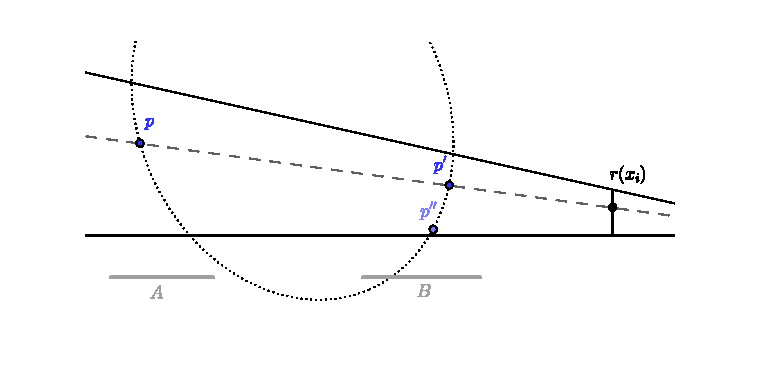
\includegraphics[width=.8\textwidth]{fig/pp_projection.pdf}
\label{fig:pp_projection}
\caption{Illustration of point cloud to range image projection in 2D}
\end{figure}

A simple approach to define the function $r$ is to let $r(x_i, y_i)$ be the point in $P_{(x_i,y_i)}$ that is closest to the camera, or $\epsilon$ when $P_{(x_i,y_i)}$ is empty. If $P_{(x_i,y_i)}$ was not a discrete set, but instead an uncountable set of surface points, it would be guaranteed that the chosen point $p$ if not occluded by another point $p'$ lying in front of it, because $p'$ would necessarily also be in $P_{(x_i,y_i)}$.

Choosing the closest point is not necessarily the best approach. Another point $p''$ might be a better candidate, when evaluating additional attributes of the points. Also the closest point may be an outlier located in front of $B$. Another approach can be to group several points and generate a new one. The important thing is that the point lies on surface $B$.

But because $P_{(x_i,y_i)}$ are discrete sets, if the point density is not high enough, it can occur that no point in it lies on surface $B$, and so instead one in $A$ would be chosen.



\subsection{Meshing}



\subsection{Downsampling}



\subsection{Filtering}


\subsection{Registration} \label{sec:pc_registration}
Given two point clouds $P$ and $Q$ that represent the same object, find a translation and rotation that will put both point clouds into the same coordinate system, and thus align the corresponding parts. $P$ and $Q$ are be taken from different poses, so different parts of the object are occluded in the two point clouds.

For example to obtain a full point cloud of a solid object, it needs to be scanned from different sides. Before it can be merged into a full point cloud, the precise relative poses of the scans need to be known. The aim of a registration algorithm is to compute an estimation of those poses.

Many different methods exist. A large survey of registration methods is given in chapter \ref{ch:pcreg}.



\subsection{Image-to-cloud registration}



\section{Data structures for point clouds}
Even though a point cloud is defined as an unordered set of points, for it to be processed algorithmically the data needs to be laid out in a certain way in computer memory. The lack of an order relation between the points provides for great flexibility. At the same time, the structure of a point cloud is that of a sparse discrete set of points embedded in three-dimensional continuous space, whereas computer memory is a dense, discrete array of bits.

Compromises need to be made in laying out the data in a way such that the required operations can be performed efficiently. 




\section{Preliminary mathematics}
This section presents some mathematical results and methods that are used in the text to follow.

\subsection{Transformation matrices and homogeneous coordinates}
Positions in three-dimensional space can be represented using cartesian coordinates. Let $O$ be an origin point in space, and let $\vec{i}, \vec{j}, \vec{k}$ be three orthogonal vectors of norm $1$. Then $\vec{p} = (x, y, z)$ represents the position $O + x \, \vec{i} + y \, \vec{j} + z \, \vec{k}$. The vectors $\vec{o}, \vec{i}, \vec{j}, \vec{k}$ define the coordinate system.

A point cloud as defined as a set of points, where each one has a position and possible additional attributes. The positions in one point cloud are all set in the same coordinate system. When the points are attributes with normal vectors, or other vector-type attributes, this is also true for them. Applying a transformation $\matr{T}$ to a point cloud means applying that transformation to the position, and if applicable to any vector-type attributes of it.

\subsubsection{Classification}
The transformations used here are classified as follows:

\begin{figure}[h]
\center
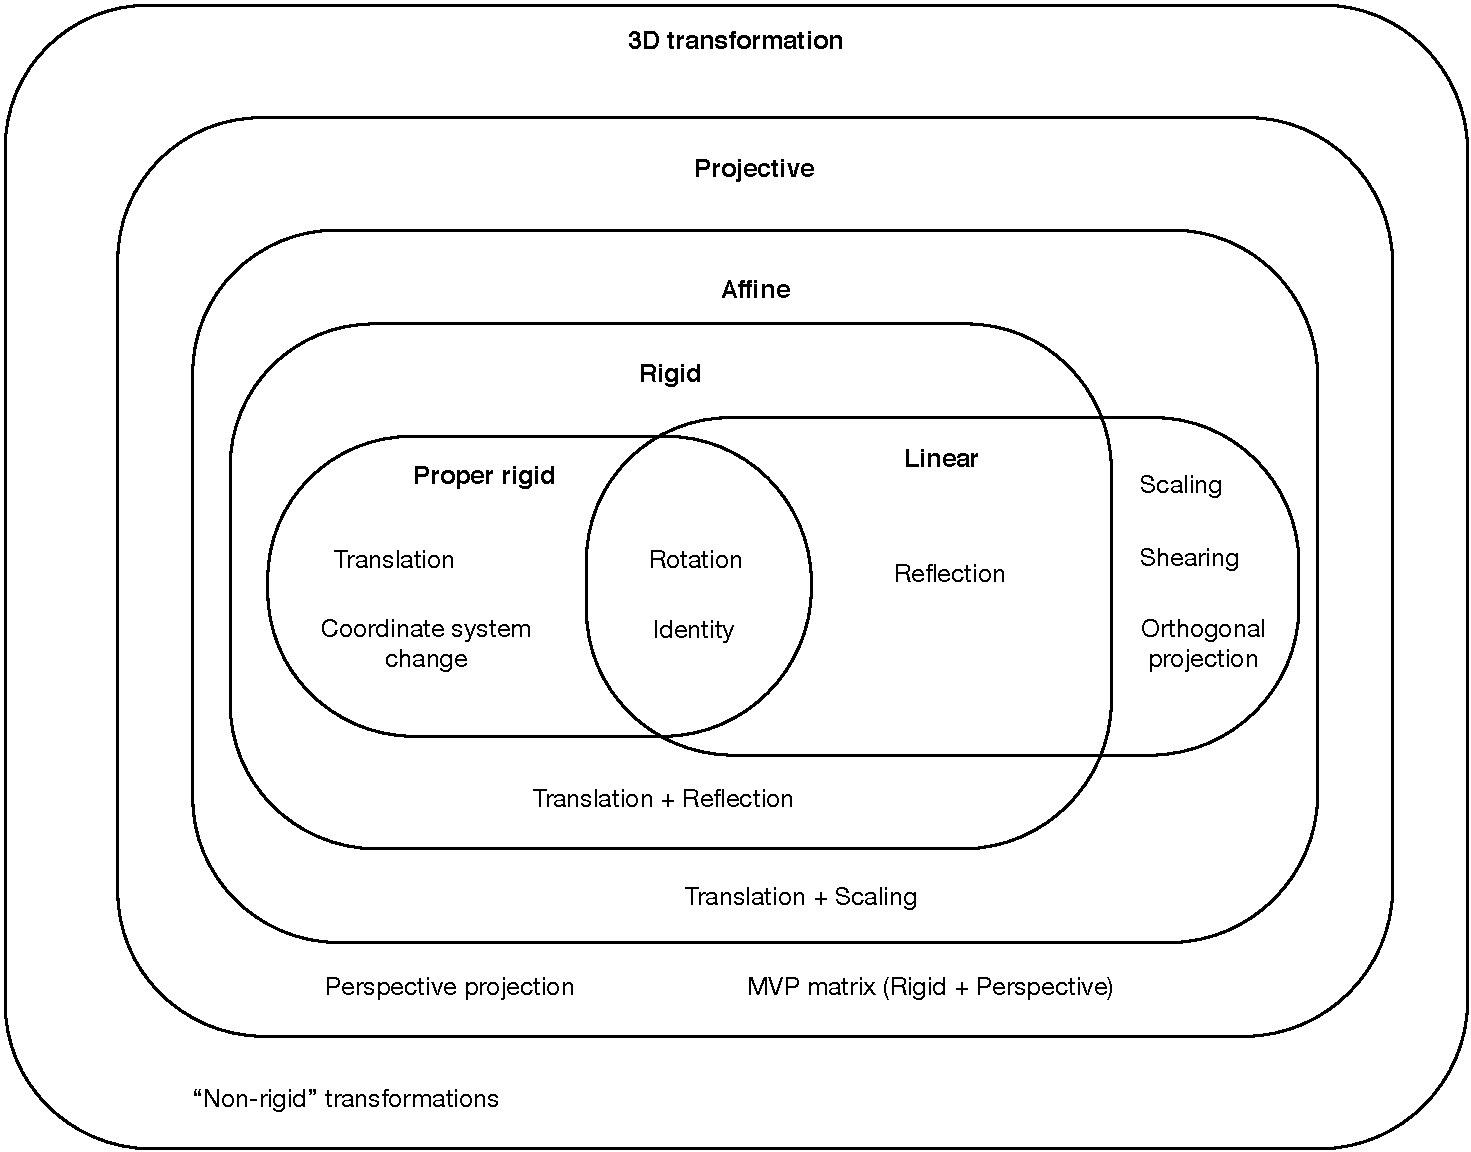
\includegraphics[width=.8\textwidth]{fig/transformations_venn.pdf}
\caption{Venn diagram of three-dimensional transformations}
\end{figure}

\emph{Linear} transformations correspond to a linear recombination of the three coordinates, and can be expressed using a $3 \times 3$ transformation matrix. \emph{Affine} transformations are linear transformation with an additional translation. A \emph{rigid} transformation is an affine transformation where the linear part corresponds to an orthogonal matrix. It preserves the distance between every pair of points. \emph{Proper rigid} transformations exclude shearing, and consist of a rotation and a translation. They correspond to the movement an object can make in three-dimensional space without altering its shape. A \emph{projective} transformation is an affine transformation, followed by a division of the three coordinates by one same linear combination of the coordinates. It can for instance express perspective projections. Additionally, the term \emph{non-rigid} transformation is sometimes used in the context of point cloud registration, to express any transformation (not necessarily affine) that alters the shape of the model.

Transformations can be combined into a conjunction of transformations, which would be classified into the lowest common class of its components. For instance a translation followed by a reflection would be a rigid transformation that is neither linear nor proper rigid. Conjunctions of transformations are in general not commutative, but all possible orders of application belong to the same class.

\subsubsection{Linear transformation}
A linear transformation is one where each coordinate of a point is mapped to a linear combination of the three coordinates. As such it can be expressed using a $3 \times 3$ matrix, and applying the transformation corresponds to multiplying this matrix $\mat{T}$ by column vector formed by the point coordinates.
\begin{equation}
\left[ \begin{matrix}
	t_{1,1} & t_{1,2} & t_{1,3} \\
	t_{2,1} & t_{2,2} & t_{2,3} \\
	t_{3,1} & t_{3,2} & t_{3,3}
\end{matrix} \right] \times
\left[ \begin{matrix} x \\ y \\ z \end{matrix} \right] = 
\left[ \begin{matrix}
	t_{1,1} \, x + t_{1,2} \, y + t_{1,3} \, z \\
	t_{2,1} \, x + t_{2,2} \, y + t_{2,3} \, z \\
	t_{3,1} \, x + t_{3,2} \, y + t_{3,3} \, z
\end{matrix} \right]
\end{equation}
So in a transformation $\vec{p'} = \matr{T} \, \vec{p}$, $t_{i,j}$ indicates the coefficient of the $j$-th coordinate of $\vec{p}$ in the $i$-th coordinate of $\vec{p'}$. As a consequence the origin $(0, 0, 0)$ is a fixed point in linear transformation. Linear transformations can for example express a rotation, a shearing, a reflection, or an orthogonal projection. Because of the associativity of matrix multiplication, the composition of linear transformations can be expressed in one single linear transformation matrix. First applying $\matr{T_1}$ followed by $\matr{T_2}$ is the same as applying $\matr{T_2} \times \matr{T_1}$, because
\begin{equation}
	\vec{p'} = \matr{T_2} \, ( \matr{T_1} \, \vec{p} ) = (\matr{T_2} \, \matr{T_1}) \, \vec{p}
\end{equation}

Also, the inverse transformation is expressed by the inverse of the transformation matrix $\matr{T^{-1}}$. As mentioned, the conjunction of two linear transformations is non-commutative, just like the underlying matrix multiplication.

\subsubsection{Rotation}
In two dimensional euclidian geometry, a rotation around the origin point $(0, 0)$ with angle $\theta$ is expressed by the linear transformation matrix
\begin{equation}
\matr{R}_{\theta} = \left[ \begin{matrix}
	\cos \theta & - \sin \theta \\
	\sin \theta & \cos \theta
\end{matrix} \right]
\label{eq:rotation-matrix-2d}
\end{equation}
This can be derived using the geometric definition of the trigonometric functions. In three-dimensional additionally a plane of rotation, of equivalently an axis of rotation needs to be specified. The linear transformation matrices for the \emph{elemental rotations} around the \emph{x}, \emph{y} or \emph{z} axis can be deduced from \ref{eq:rotation-matrix-2d} by keeping one coordinate unchanged and applying the 2D rotation on the plane formed by the other two:
\begin{equation}
\matr{R}_{\theta}^x = \left[ \begin{matrix}
	1 & 0 & 0 \\
	0 & \cos \theta & - \sin \theta \\
	0 & \sin \theta & \cos \theta
\end{matrix} \right]
\hspace{1cm}
\matr{R}_{\theta}^y = \left[ \begin{matrix}
	\cos \theta & 0 & \sin \theta \\
	0 & 1 & 0 \\
	- \sin \theta & 0 & \cos \theta
\end{matrix} \right]
\hspace{1cm}
\matr{R}_{\theta}^z = \left[ \begin{matrix}
	\cos \theta & - \sin \theta & 0 \\
	\sin \theta & \cos \theta & 0 \\
	0 & 0 & 1
\end{matrix} \right]
\end{equation}

\subsubsection{Euler angles}
One common way to express a three-dimensional rotation is using \emph{Euler angles}, that is, the angles by which to rotate around those three axis. For example, $(\phi, \theta, \psi)$ may express the rotation $\matr{R}_{\phi}^x \, \matr{R}_{\theta}^y \, \matr{R}_{\psi}^z$. Because of the non-commutativity, many different conventions are possible: The three elementary rotations can be applied in different orders, such as \emph{x-y-z}, \emph{z-y-x} or \emph{x-y-z}. Also combinations of only two elementary rotations like \emph{x-y-x} or \emph{z-x-z} are possible, where the same axis used for the first and third rotation. In expression like $\matr{R}_{\phi}^x \, \matr{R}_{\theta}^y \, \matr{R}_{\psi}^z$, the three elementary rotations are \emph{intrinsic}: The second rotation rotates around the new \emph{y} axis, which has already been displaced from the first rotation. In an \emph{explicit} conventions, all three rotations instead take place in a fixed coordinate system.

The terms \emph{yaw}, \emph{pitch} and \emph{roll} are commonly used to name the three rotation angles. Given an object pointing into a certain direction in space, such as a camera or a moving vehicle, \emph{roll} refers to a rotation around the axis in which it is pointing. \emph{Pitch} is a rotation around its relative horizontal axis, and \emph{yaw} around its relative vertice axis. For example, a \emph{pitch} rotation of an aircraft would make it fly upwards or downwards.

Besides the many possible conventions, another problem with Euler angles is the \emph{gimbal lock} phenomenon, where two components can end up representing a rotation around the same axis.

Because of gimbal lock, and because the angles are taken modulo $2\pi$, small changes in a rotation do not always correspond to small changes in the Euler angles. This makes them unsuited for processing rotations algorithmically and for solving optimisation problems. Instead, a good alternative to directly working with rotation matrices is to use quaternions, which express the rotation using $4$ real values.

\subsubsection{Quaternions}
...

\subsubsection{Rotation around an axis}

\subsubsection{Rotation between two vectors}

\subsubsection{Affine transformation}
Translations are not linear transformations, because they add a constant term to each coordinate of $\vec{p'}$. An \emph{affine} transformation corresponds to a linear transformation followed by a translation: $\vec{p'} = \matr{T} \, \vec{p} + \vec{t}$. Let $\vec{p'} = \matr{T_1} \, \vec{p} + \vec{t_1}$ and $\vec{p''} = \matr{T_2} \, \vec{p'} + \vec{t_2}$ be the expressions of two subsequent affine transformation to apply to $\vec{p}$.
\begin{equation}
	\vec{p''} = \matr{T_2} \, (\matr{T_1} \, \vec{p} + \vec{t_1}) + \vec{t_2} = (\matr{T_2} \, \matr{T_1}) \, \vec{p} + (\matr{T_1} \vec{t_1} + \vec{t_2})
\end{equation}
So a composition of multiple affine transformations is still an affine transformation, but the translation vectors cannot be simply added up. It can be seen that the composition is again non-commutative, except for the case when $\matr{T_2} = \matr{T_1} = \matr{I}$, that is, when both transformations are translations only.

Also if the translation component is applied \emph{before} the linear component (instead of \emph{after} it), it represents a different affine transformation:
\begin{equation}
	\matr{T} \, (\vec{p} + \vec{t}) = \matr{T} \, \vec{p} + \matr{T} \, \vec{t} \neq \matr{T} \, \vec{p} + \vec{t}
\end{equation}

\subsubsection{Rigid transformation}
The subclass of affine transformation where $\matr{T}$ is an orthogonal matrix are the rigid transformations. By definition, its row vectors, and its column vectors are orthogonal unit vectors. Orthogonal matrices preserve the dot product of vectors, and as a consequence distances and angles between any two pairs of points are preserved. Orthogonal matrices represent either a rotation or a reflection, and its determinant $\det(\matr{T})$ is always either $+1$ for a rotation or $-1$ for a reflection. This is a necessary but not sufficient condition, as there are also non-orthogonal matrices with determinant $+1$ or $-1$. So a rigid transformation can be a translation, rotation, reflection, or any composition thereof.

A proper rigid transformation is defined as a rigid transformation for which $\matr{T}$ is a rotation matrix. It always consists of a rotation and a translation, and any composition of proper rigid matrices can be reformulated as a single rotation and translation:
\begin{equation}
	\matr{R_2} \, (\matr{R_1} \, \vec{p} + \vec{t_1}) + \vec{t_2} = (\matr{R_2} \, \matr{R_1}) \, \vec{p} + (\matr{R_2} \, \vec{t_1} + \vec{t_2})
\end{equation}
Where $\matr{R_2} \, \matr{R_1}$ is also an orthogonal matrix, it being the composition of two rotations.

Proper rigid transformations correspond to the ways a real object can be moved in three-dimensional space without altering its shape. As such, they can be used to represent the position and orientation of an object.

In the following text, the term ``rigid transformation'' will always refer to a proper rigid transformation.

In most use cases involving three-dimensional geometry, non-proper rigid transformations are rarely used since they change the handedness of an object, which is in reality not possible in three-dimensional space. In fact, with a fourth spatial dimension it would be possible with a 4D rotation that temporarily pulls the object out of the three-dimensional subspace. This process would not alter the object's internal structure. But while both the start and end state would be possible in 3D space, the intermediary steps are not, and movements in reality are always continuous.

\subsubsection{Homogeneous coordinates}
In order to simplify calculations and notation, it is natural to use \emph{homogeneous coordinates}. They allow for affine and projective transformations to be written using a single $4 \times 4$ matrix.

Formally, a vector $\homvec{v}$ in homogeneous coordinates corresponds to a vector $\vec{v}$ in cartesian coordinates iff
\begin{equation}
	\homvec{v} = \colvecT{x, y, z, w}
	\hspace{1cm}\mathrm{and}\hspace{1cm}
	\vec{c} = \colvecT{\frac{x}{w}, \frac{y}{w}, \frac{z}{w}}
\end{equation}

The conversion from homogeneous to cartesian coordinates consists of an element-wise division by the fourth component $w$ of the vector itself. This non-linear operation cannot be represented by cartesian matrix multiplications alone. The equivalent in homogeneous coordinates of an affine transformation given by the linear transformation $\matr{L}$\footnote{Using $\matr{L}$ here instead of $\matr{T}$ to have different lowercase letters.}, and the translation vector $\vec{t}$, where the linear transformation is applied before the translation, is the $4 \times 4$ matrix
\begin{equation}
	\hommatr{T} = \left[ \begin{matrix}
		l_{1,1} & l_{1,2} & l_{1,3} & t_1 \\
		l_{2,1} & l_{2,2} & l_{2,3} & t_2 \\
		l_{3,1} & l_{3,2} & l_{3,3} & t_3 \\
		0 & 0 & 0 & 1
	\end{matrix} \right]
\end{equation}
A distinction is made between positions and vectors: When transforming a position, with the linear transformation is applied, followed by the translation. For vectors on the other hand, only the linear transformation is applied. A vector does not have a position in space, but only a direction and norm. Its coordinates represent the position of its end point, assuming that its start point is at $\colvecT{0, 0, 0}$. For example when applying a rigid transformation to a point cloud where points are attributed with surface normal vectors, the point positions should get rotated and then translated. The normal vectors should be rotated the same way, but no translation vector should be added to them.

Positions are converted into homogeneous coordinates by adding an extra component $w = 1$, whereas for vectors an extra component $w = 0$ is added. The three first components $x, y, z$ remain the same. It can be seen that
\begin{equation}
\left[ \begin{matrix}
	x \\ y \\ z \\ 1
\end{matrix} \right] \times  \left[ \begin{matrix}
	l_{1,1} & l_{1,2} & l_{1,3} & t_1 \\
	l_{2,1} & l_{2,2} & l_{2,3} & t_2 \\
	l_{3,1} & l_{3,2} & l_{3,3} & t_3 \\
	0 & 0 & 0 & 1
\end{matrix} \right] = \left[ \begin{matrix}
	l_{1,1} \, x + l_{1,2} \, y + l_{1,3} \, z + t_1 \\
	l_{2,1} \, x + l_{2,2} \, y + l_{2,3} \, z + t_2 \\
	l_{3,1} \, x + l_{3,2} \, y + l_{3,3} \, z + t_3 \\
	1
\end{matrix} \right] \coreq \left[ \begin{matrix}
	l_{1,1} \, x + l_{1,2} \, y + l_{1,3} \, z + t_1 \\
	l_{2,1} \, x + l_{2,2} \, y + l_{2,3} \, z + t_2 \\
	l_{3,1} \, x + l_{3,2} \, y + l_{3,3} \, z + t_3 \\
\end{matrix} \right]
\end{equation}
In the case where $w = 0$, the components of $\vec{t}$ get removed. In the case of affine transformations, the last row of the homogeneous matrix is always $\rowvec{0, 0, 0, 1}$, and no division takes place. For perspective projections, a division by the $z$ component will compute foreshortening.

Because here an affine or projective transformation is applied by single matrix multiplication, is follows that any composition of those matrices can be represented using the matrix product of multiple $4 \times 4$ matrices.

\subsubsection{Pose}
This position and orientation of an object in space is called its \emph{pose}. A pose is also a cartesian coordinate system. Coordinates as well as other poses are always defined relative to such a coordinate system.

In any sufficiently complex three-dimensional environment, it becomes natural to define the positions and orientations of object relative to each other, and not in a single global coordinate system. 3D modelling software such as \emph{Blender} typically implement a tree-structure of objects, in which the pose of each object is defined relative to its parent. A similar software system was written for this project.

The problem of 3D scan registration treated in this paper is precisely to find the pose from which a scan was taken, relative to another scan, and the output of any point cloud registration algorithm is a rigid transformation matrix.

A pose corresponds to an orthonormal coordinate system which is defined by tuple $S = \langle O, \vec{i}, \vec{j}, \vec{k} \rangle$ where $O$ is the origin point, and $\vec{i}, \vec{j}, \vec{k}$ three orthogonal vectors with $\|\vec{i}\| = \|\vec{j}\| = \|\vec{k}\| = 1$. The origin point and the vectors of a coordinate system are defined within its \emph{parent} coordinate system. The root coordinate system in that tree is called \emph{world space}. For an \emph{identity} coordinate system, $O = (0, 0, 0)$, $\vec{i} = \colvecT{1, 0, 0}$, $\vec{j} = \colvecT{0, 1, 0}$ and $\vec{k} = \colvecT{0, 0, 1}$.

A pose can also be expressed using the \emph{transform-to-parent} rigid transformation $\matr{M}$, which transforms the coordinates of points or vectors expressed in its coordinate system $S_i$, into the coordinates of the same point of vector in its parent coordinate system $S_{i-1}$. Equivalently, the \emph{transform-from-parent} rigid transformation is its inverse $\matr{M^{-1}}$. Then
\begin{equation}
	O_{i} = \matr{M^{-1}} \, O_{i-1}
	\hspace{1cm}
	\vec{i_{i}} = \matr{M^{-1}} \, \vec{i_{i-1}}
	\hspace{1cm}
	\vec{j_{i}} = \matr{M^{-1}} \, \vec{j_{i-1}}
	\hspace{1cm}
	\vec{k_{i}} = \matr{M^{-1}} \, \vec{k_{i-1}}
\end{equation}
where the distinction between positions and vectors using homogeneous coordinates is made.



...

\subsection{Least squares method}
The least squares method is a way to calculate an approximate solution to an overdetermined system. For example the equation $y = ax + b$ of a line that crosses two points $(x_1, y_1)$ and $(x_2, y_2)$ can easily be calculated by solving a linear system with 2 equations and 2 unknowns. But if there are 3 or more points, there is no solution unless the points are perfectly aligned. Here a least squares solution would be the line which minimizes the sum of the squares of the distances of the points to itself.

Formally, let $\{ (x_i, y_i) \}$ be a set of $n$ data points. $x_i$ are independent variables and $y_i$ dependent variables found by observation. Both $x_i$ and $y_i$ can be vectors. For example the problem of fitting a plane to a set of 3D points may be modelled with $x_i$ being a data point's X coordinate, and $\vec{y_i}$ that data point's Y and Z coordinates.

The goal is to find a vector of parameters $\beta$ that define a model $\hat{y}_i = f_{\beta}(x_i)$. Because in general there is no $f_{\beta}$ for which $\forall i, \hat{y}_i = y_i$, one searches a solution that minimizes the sum of the squared residuals:
\begin{equation}
\hat{\beta} = \argmin_{\beta} S \hspace{7mm} \text{where} \hspace{7mm} S = \sum_{i=1}^{n} (y_i - \hat{y}_i)^2
\end{equation}
For the example where the model is a line, one can define $\beta = (a, b)$ and $f_{\beta}(x) = ax + b$. Then the residual would be the vertical distance of a point to a line. It is also possible to define a linear expression of $f_{\beta}$ by which the orthogonal distances of the points to the lines is minimised. Many similar geometrical fitting problems can be solved in this manner, such as fitting a plane, circle, sphere, or other object to a set of points. \cite{Eber1999}

\subsubsection{Linear least-squares}
In general, a solution for least square problems can be computed by setting the gradient $\nambla S$ to zero. Since the terms $y_i$ are constant, this becomes for each component $\beta_j$:
\begin{equation} \label{eq:lsq_sol}
\frac{\partial S }{\partial \beta_j} = -2 \sum_{i=1}^{n} \frac{\partial f_{\beta}(x)}{\partial \beta_j} = 0
\end{equation}

If $f_{\vec{\beta}}$ is a linear combination of the parameters $\vec{\beta}$, then a closed form expression for the solution exists. Let there be $n$ data points $(x, y)$, where $x$ are vectors of $m$ components, and $y$ real numbers. (Here the subscript refers to the component of the vector $x$, not the index of the data point). $\beta$ will also have $m$ components. The function $f_{\beta}$ is of the form
\begin{equation} \label{eq:lsq_linf}
f_{\beta}(x) = \beta_1 \, x_1 + \beta_2 \, x_2 + \dots + \beta_m \, x_m
\end{equation}
For the example of fitting a line to a set of 2D points, one would add a second component to the dependent variables which is always set to $1$, so as to get back to $f_{\beta}(x) = ax + b$.

The overdetermined system to solve can be written in matrix form
\begin{equation}
\matr{X} \, \hat{\beta} = \vec{y}
\end{equation}
where $\matr{X}$ is a $n \cross m$ matrix. Each row corresponds to a data point, and each component per row corresponds to the $j$-th component $x_j$ of the dependent variable of that data point. The sum of squares $S$ to minimize becomes
\begin{equation}
S = \sum_{i=1}^{n} \| y_i - \sum_{j=1}^{m} X_{i,j} \beta_{j} \|^2 = \| y - \matr{X} \, \vec{\beta} \|^2
\end{equation}
From \ref{eq:lsq_linf}, the partial derivative of a residual becomes
\begin{equation} \label{eq:lsq_linr}
\frac{\partial (y_i - f_{\beta}(x))}{\partial \beta_j} = - X_{i,j}
\end{equation}
Putting \ref{eq:lsq_linr} into \ref{eq:lsq_sol} and rearranging the expression, one obtains the \emph{normal equations}:
\begin{equation}
\sum_{i=1}^{n} \sum_{k=1}^{m} X_{ij} \, X_{ik} \, \hat{\beta}_k = \sum_{i=1}^{n} X_{ij} \, y_{i}
\hspace{7mm} \text{for} \hspace{7mm}
j = 1, 2, \dots, m
\end{equation}
Written in matrix form:
\begin{equation}
(\transpose{\matr{X}} \, \matr{X}) \, \hat{\beta} = \transpose{\matr{X}} \, \vec{y}
\end{equation}
And so the parameters $\hat{\beta}$ for which $f_{\hat{\beta}}(x)$ is a least squares solution to a linear system can be computed using the closed form expression
\begin{equation}
\hat{\beta} = (\transpose{\matr{X}} \, \matr{X})^{-1} \, \transpose{\matr{X}} \, \vec{y}
\end{equation}

\subsubsection{Non-linear least squares}
When $f_{\beta}$ is not a linear combination of $x_1, x_2, \dots, x_m$ a closed form solution is generally not possible. Instead it can be computed using the \emph{Gauss-Newton algorithm}, by iterative numerical approximation.

\subsubsection{Weights}
The least squares methods finds a solution for which the squared residual $(y_i - \hat{y}_i)^2$ is minimized and evenly distributed among all data points. Weights can be added to introduce bias towards higher weight data points, letting their residual become smaller and the others' larger.

For each data point a \emph{weight} $w_i \in \mathds{R}$ is defined. When $w_i = k \times w_j$ for $k \in \mathds{N}$, the effect is the same as adding $k$ times the data point $(x_i, y_i)$. With weights, the sum to minimize is
\begin{equation}
S = \sum_{i=1}^{n} w_i \, (y_i - \hat{y}_i)^2
\end{equation}
By distributivity, when all $w_i$ become $\lambda w_i$, $S$ becomes $\lambda S$, which doesn't change the minimization problem. Supposing that $w_i$ are rational numbers (which can approximate real numbers to an arbitrary precision), then there exists $\lambda$ such that $\lambda w_i \in \mathds{N}$. This justifies the previous statement about data points duplication. 

\subsubsection{}

\subsection{Point set alignment using singular value decomposition} \label{sec:lsq_align}
For point cloud registration, corresponding points $(\vec{p_i}, \vec{q_i})$ of two point clouds are used to find a rigid transformation $\matr{M}$ that aligns the two point clouds. When there are exactly three pairs of points, an exact solution can be found using vector algebra. \cite{Horn1986} For more than three points, a least squares solution can be found.

Here $f_{\beta}(\vec{q}) = \matr{M} \, \vec{q} = \matr{R} \, \vec{q} + \vec{t}$ is the function that applies the sought after rigid transformation. The parameter vector $\beta$ has 6 components, three for the translation and three for the rotation. $\matr{R}$ is the rotation matrix and $\vec{t}$ the translation vector. The independent variable is $\vec{q_i}$, a 3-vector with the coordinates of a point. The dependent variable is $\vec{p_i}$, also a 3-vector with the coordinates of the corresponding point from the other point cloud.

Because the independent variables are vectors, the residuals to minimize are the squares of the norms of the vector differences. The sum $S$ to minimize becomes
\begin{equation}
S = \sum_{i=1}^{n} w_i \, \| \vec{p_i} - (\matr{R} \, \vec{q_i} + \vec{t}) \|^2
\end{equation}

The assumption is that both point sets $\{ p_i \}$ and $\{ q_i \}$ have approximately the same constellation but are in a different pose. For registration, first they need to be translated so as to make one common point coincide, and then they can be aligned by rotating one point set around that point. As a common point, the centroids of both point clouds are chosen:
\begin{equation}
\vec{c_p} = \frac{1}{N} \, \sum_{i=1}^{n} \vec{p_i}
\hspace{7mm} \text{and} \hspace{7mm}
\vec{c_q} = \frac{1}{N} \, \sum_{i=1}^{n} \vec{q_i}
\end{equation}
Because the constellations are not exactly equal, this choice evenly distributes the error. Also, when the shape that the points form around the centroid point is roughly that of a sphere (their distances from the centroid do not vary too much), the rotating around the centroid will move each point by about the same amount, again evening out the error. 

A rotation matrix $\matr{R}$ expressed a rotation around the origin. In order to simplify the problem, both point clouds are first translated to put the centroid at origin. So $\forall i$ one defines
\begin{equation}
\vec{p'_i} = \vec{p_i} - \vec{c_p}
\hspace{7mm} \text{and} \hspace{7mm}
\vec{q'_i} = \vec{q_i} - \vec{c_q}
\end{equation}
and the minimization problem becomes
\begin{equation} \label{eq:lsq_align_meaneds}
S' = \sum_{i=1}^{n} w_i \, \| \vec{p'_i} - \matr{R} \, \vec{q'_i} \|^2
\end{equation}
Since $\vec{t}$ was applied after $\matr{R}$, this does not change the meaning of $\matr{R}$.

Different approaches exist for computing $\matr{R}$ in constant time, that is without the need for iterative numerical approximation. \cite{Horn1986} describes a solution whereby $\matr{R}$ is represented as a unit quaternion. This was used in the original description of the ICP algorithm (see \label{sec:icp}) in \cite{Besl1992}. \cite{Loru1995} gives a comparison of four methods, also in the context of the ICP algorithm. Probably the most commonly implemented approach is the following, which is based on singular value decomposition.

Using some matrix algebra, \ref{eq:lsq_align_meaneds} becomes
\begin{equation}
S' = \sum_{i=1}^{n} w_i \, \| \vec{p'_i} \|^2 + w_i \, \| \vec{q'_i} \|^2 - 2 \, w_i \, \transpose{\vec{q'_i}} \, \matr{R} \, \vec{p'_i}
\end{equation}
The first and second terms do not depend on $\matr{R}$, hence the problem is reduced to maximizing $\sum_{i} w_i \, \transpose{\vec{q'_i}} \, \matr{R} \, \vec{p'_i}$.

Let $\matr{W} = \text{diag}(w_1, w_2, \dots, w_n)$, and let $\matr{P}$ and $\matr{Q}$ be $3 \times n$ matrices composed of the $n$ column-vectors. One has
\begin{equation}
\matr{W} \, \transpose{\matr{Q}} = \left[ \begin{matrix}
	\-- & w_1 \, \transpose{\vec{q'_1}} & \--\\
	\-- & w_2 \, \transpose{\vec{q'_2}} & \--\\
	& \vdots & \\
	\-- & w_n \, \transpose{\vec{q'_n}} & \--
\end{matrix} \right]
\hspace{7mm} \text{and} \hspace{7mm}
\matr{R} \, \matr{P} = \left[ \begin{matrix}
	| & | & & |\\
	\matr{R} \, \vec{p'_1} & \matr{R} \, \vec{p'_2} & \hdots & \matr{R} \, \vec{p'_n}\\
	| & | & & |
\end{matrix} \right]
\end{equation}
It can be seen that
\begin{equation}
\sum_{i=1}^{n} w_i \, \transpose{\vec{q'_i}} \, \matr{R} \, \vec{p'_i} = \text{tr}(\matr{W} \, \transpose{\matr{Q}} \, \matr{R} \, \matr{P})
\end{equation}
Where the trace $\text{tr}$ is the sum of the diagonal entries of a matrix. Because $\matr{A} \matr{B} = \transpose{(\matr{B} \matr{A})}$ and the trace is invariant under the transpose,
\begin{equation}
\text{tr}((\matr{W} \, \transpose{\matr{Q}}) \, (\matr{R} \, \matr{P})) = \text{tr}((\matr{R} \, \matr{P}) \, (\matr{W} \, \transpose{\matr{Q}})) = \text{tr}(\matr{K} \, \matr{R})
\end{equation}
This $n \times n$ \emph{covariance matrix}\footnote{Also called \emph{correlation} matrix.} $\matr{K}$ can be computed directly from the input data points:
\begin{equation}
\matr{K} = \matr{P} \, \matr{W} \, \transpose{\matr{Q}} = \sum_{i=1}^{n} w_i \, \vec{p'_i} \, \transpose{\vec{q'_i}}
\end{equation}

Here the \emph{singular value decomposition} of $\matr{K}$ is taken:
\begin{equation}
\matr{K} = \matr{U} \, \matr{\Sigma} \, \transpose{\matr{V}}
\end{equation}
Now $\matr{U}$, $\matr{V}$ and also the unknown rotation matrix $\matr{R}$ are orthogonal matrices, and $\matr{\Sigma}$ is a non-negative diagonal matrix. Again using the properties of the $\text{tr}$, it can be rewritten
\begin{equation}
\text{tr}(\matr{K} \, \matr{R}) = \text{tr}(\matr{\Sigma} \, \transpose{\matr{V}} \, \matr{R} \, \matr{U})
\end{equation}
Now $\matr{N} = \transpose{\matr{V}} \matr{R} \matr{U}$ is also an orthogonal matrix, and so all $\| n_{i,j} \| \leq 1$. The trace $\text{tr}(\matr{\Sigma} \matr{N}) = \sum_{i} \sigma_i n_{ii}$ is maximal when $\matr{N}$ is such that $\forall i, n_{ii} = 1$, i.e. when $\matr{N} = \matr{I}$.

Solving for $\matr{R}$, one obtains:
\begin{equation}
\matr{N} = \transpose{\matr{V}} \, \matr{R} \, \matr{U} = \matr{I}
\Rightarrow \matr{V} = \matr{R} \, \matr{U}
\Rightarrow \matr{R} = \matr{V} \, \transpose{\matr{U}}
\end{equation}
The resulting $\matr{R}$ is always an orthogonal matrix, but not necessarily a rotation matrix. If $det(\matr{R}) = -1$ it is a reflection instead. This is obtained when the point sets are such that a reflection aligns them better than a rotation.

To always find a rotation a rectification step needs to be added to the algorithm: When $det(\matr{R}) = -1$, instead choose $\matr{R'}$ for which $det(\matr{R'}) = 1$ and $S'$ attains the next best possible local maximum. $\matr{R'}$ is obtained by replacing the entries of $\matr{R}$ in the third column by their opposite.

This shows how the rotation matrix $\matr{R}$ which minimizes $S'$ can be computed from the singular value decomposition of the covariance matrix $\matr{K}$. The point sets $\{ \vec{p'_i} \}$ and $\{ \vec{q'_i} \}$ have been translated to put their centroids $\vec{c_p}$ and $\vec{c_q}$ to the origin. Since adding a translational component to a rigid transformation does not change its rotational component, $\matr{R}$ is also valid on the original point sets. It remains to calculate the translation vector $\vec{t}$.

On the original point sets, $(\matr{R}, \vec{t})$ should solve $\vec{p_i} = \matr{R} \, \vec{q_i} + \vec{t}$ in a least squares sense. One has $\vec{p'_i} = \matr{R} \, \vec{q'_i}$, where $\vec{p'_i} = \vec{p_i} - \vec{c_p}$ and $\vec{q'_i} = \vec{q_i} - \vec{c_p}$. Putting this together and solving for $\vec{t}$, one obtains
\begin{equation}
\vec{t} = \vec{c_p} - \matr{R} \, \vec{c_q}
\end{equation}


\subsection{Information theory}

\subsection{Gaussian distribution}

\subsection{Parzen window}

\subsection{RANSAC}

\section{Preliminary computer science}

\subsection{Octree}

\subsection{KdTree}
